\documentclass[]{article}
\usepackage[a4paper, total={6in, 10in}]{geometry}
\usepackage{hyperref}
\usepackage{amsmath}
\usepackage{graphicx}
\usepackage[outdir=./]{epstopdf}
\usepackage{booktabs}
\usepackage{float}
\usepackage{subcaption}

\setlength{\parindent}{0em}
\setlength{\parskip}{1em}

\DeclareMathOperator{\cov}{cov}

%opening
\title{SSY 230, System Identification\\
	Project 1: Estimating functions from noisy data}
\author{Yuxuan Xia\\ \href{mailto:yuxuan.xia@chalmers.se}{yuxuan.xia@chalmers.se}\\Emil Staf\\\href{mailto:emil.staf@chalmers.se}{emil.staf@chalmers.se}}

\begin{document}

\maketitle

\section{Linear regression functions}

\subsection{Estimation parameter validation}
Verifying the parameter estimates and the uncertainty of the estimates requires some calculations by hand. In matrix form the parameter estimate is given by
\begin{equation}
	\label{eq:estimate}
	\hat{\theta} = (X^\mathsf{T}X)^{-1}X^\mathsf{T}Y
\end{equation}
where $X$ is the regressor matrix and $Y$ is the dependant variables. The uncertainty is given by
\begin{equation}
	\label{eq:estimate_cov}
	\cov(\hat{\theta}) = \lambda^2(X^\mathsf{T}X)^{-1}
\end{equation}
with $\lambda^2$ is the variance of the signal noise. Since $\lambda^2$ is unknown it has to be estimated using the data and an unbiased estimate is given by
\begin{equation}
	\label{eq:s2}
	s^2 = 2*V(\hat{\theta})/(N-n)
\end{equation}
where $N$ is the number of feature vectors, $n$ is the number of regressor dimensions and $V(\hat{\theta})$ is given by
\begin{equation}
	\label{eq:error}
	V(\hat{\theta}) = \frac{1}{2}[Y-X\theta]^\mathsf{T}[Y-X\theta].
\end{equation}
The verification data is given by 

\begin{equation}
	X = \begin{bmatrix}
	1 & 1 \\
	1 & 2 \\
	1 & 3
	\end{bmatrix},
	Y = \begin{bmatrix}
	1.1 \\
	1.8 \\
	3.1
	\end{bmatrix}.
\end{equation}
Using \eqref{eq:estimate} it is easy to verify that the estimate is $\hat{\theta} = [0, 1]^\mathsf{T}$. Using the found estimate \eqref{eq:error} gives $V(\hat{\theta})=0.03$, which is used in \eqref{eq:s2} together with $N=3$ and $n=2$ and gives $s^2=0.06$. Now the covariance of the estimates is found using \eqref{eq:estimate_cov} with $s^2=0.06$ and
\begin{equation}
	(X^\mathsf{T}X)^{-1} = \begin{bmatrix}
	3 & 6 \\
	6 & 14 
	\end{bmatrix}^{-1}=\frac{1}{3\cdot14-6\cdot6}\begin{bmatrix}
	14 & -6 \\
	-6 & 3 
	\end{bmatrix} = \begin{bmatrix}
	\frac{7}{3} & -1 \\
	-1 & \frac{1}{2} 
	\end{bmatrix}.
\end{equation}
This gives an estimated covariance of 
\begin{equation}
	s^2(X^\mathsf{T}X)^{-1} = 0.06\begin{bmatrix}
	\frac{7}{3} & -1 \\
	-1 & \frac{1}{2} 
	\end{bmatrix}.
\end{equation}

\subsection{Regularization verification}

The loss function used in linear regression, using matrix notation, is
\begin{equation}
	\label{eq:loss_function}
	V_\lambda(\theta; X,Y) = \frac{1}{2}[(Y-X\theta)^\mathsf{T} (Y-X\theta) + \lambda\theta^\mathsf{T}\theta]
\end{equation}
where $\lambda$ is the regularization parameter and 
\begin{equation}
	X = \begin{bmatrix}
	| & | &  & | \\
	x_1 & x_2 & \cdots & x_d\\
	| & | &  & |\\
	\end{bmatrix},
	Y = \begin{bmatrix}
	y_1 \\
	y_2 \\
	\vdots \\
	y_N
	\end{bmatrix}
\end{equation}
where $X \, (N \times d)$, $Y\, (N \times m)$.
Verify that $V_\lambda(\theta; X, Y)$ in \eqref{eq:loss_function} is the same as $V_0(\theta; X_2, Y_2)$, where
\begin{equation}
	X_2  = \begin{bmatrix}
	X\\
	\Lambda
	\end{bmatrix},
	\Lambda = \begin{bmatrix}
	\sqrt{\lambda} & 0 & 0 \\
	0 & \ddots & 0 \\
	0 & 0 & \sqrt{\lambda} \\
	0 & 0 & 0 \\
	\vdots & \vdots & \vdots
	\end{bmatrix}
	Y_2 = \begin{bmatrix}
	y_1 \\
	y_2 \\
	\vdots \\
	y_N \\
	0\\
	\vdots
	\end{bmatrix}
\end{equation}
where $X_2 \, (2N \times d)$, $Y_2\, (2N \times m)$.

\begin{align}
V_0(\theta; X_2, Y_2) &=\frac{1}{2}(Y_2-X_2\theta)^\mathsf{T} (Y_2-X_2\theta)  = \frac{1}{2}\begin{bmatrix}
Y-X\theta\\
\mathbf{0}-\Lambda\theta
\end{bmatrix}^\mathsf{T}
\begin{bmatrix}
Y-X\theta\\
\mathbf{0}-\Lambda\theta
\end{bmatrix} = \\
&= \frac{1}{2}[(Y-X\theta)^\mathsf{T}(Y-X\theta) + (\Lambda\theta)^\mathsf{T}(\Lambda\theta)] = \frac{1}{2}[(Y-X\theta)^\mathsf{T} (Y-X\theta) + \lambda\theta^\mathsf{T}\theta].
\end{align}

Given a regressor matrix $X$ and an output matrix $Y$, the linear least squares estimate with L2-Regularization can be obtained by minimizing the sum of squared residuals,
\begin{equation}{\label{LSestimator}}
\hat{\theta} = \arg\min\limits_{\theta}(Y-X\theta)^T(Y-X\theta)+\lambda\theta^T\theta.
\end{equation}
The estimate $\hat{\theta}$ can be found by setting the derivative of (\ref{LSestimator}) w.r.t. $\theta$ to zero,
\begin{subequations}\label{LSderivative}
		\begin{align}
		\frac{d}{d\theta}\left((Y-X\theta)^T(Y-X\theta)+\lambda\theta^T\theta \right) &= 0,\\
		-X^TY+X^TX\theta+\lambda\theta &=0,\\
		(X^TX+\lambda I)^{-1}X^TY &=\hat{\theta}.
		\end{align}
\end{subequations}
It is easy to verify that, when $\lambda=0$, $\hat{\theta}$ is equal to the linear least squares estimate without regularization, i.e.,
\begin{equation}
\hat{\theta} = (X^TX)^{-1}X^TY,
\end{equation}
and that, when $\lambda\rightarrow +\infty$, $\hat{\theta}\rightarrow \mathbf{0}$.


\subsection{Polynomial fitting validation}

\begin{figure}[ht]
	\centering
	\includegraphics[trim= 10cm 5cm 10cm 5cm, scale=0.4]{proj1-1d}
	\caption{Estimated function using polynomial fitting. Each sample of regressor vector $\mathbf{x}$ is randomly drawn from uniform distribution $[0,10]$. The true function is $\mathbf{y}=1+5\mathbf{x} + 0.5\mathbf{x}^2 - 0.1\mathbf{x}^3$, the noise variance is set to 1, and the number of samples is 20. }
	\label{fig:poly1d}
\end{figure}

The estimated 3rd degree polynomial in Figure \ref{fig:poly1d} is given by $\hat{y} = 0.4 + 5.56x + 0.41x - 0.096x$, close to the true function $y=1+5x + 0.5x^2 - 0.1x^3$.

\subsection{(e) One dimensional model plotting}
\begin{figure}[H]
	\centering
	\includegraphics[trim= 10cm 5cm 10cm 5cm, scale=0.4]{proj1-1e}
	\caption{Estimated function using linear regression (LR). Uncertainty is illustrated as the region between the two dotted lines with confidence level 0.95. Each sample of regressor vector $x$ is randomly drawn from uniform distribution $[0,10]$. The true function is $y=2+2x$, the noise variance is set to 2, and the number of samples is 20. }
	\label{fig:confidence}
\end{figure}

\section{KNN-regression functions}
The implemented KNN regressor is compared against linear regression in Figure \ref{fig:KNNvsLR}.
\subsection{KNN v.s. Linear regression}
\begin{figure}[ht]
	\centering
	\includegraphics[trim= 10cm 5cm 10cm 5cm, scale=0.4]{proj1-2c}
	\caption{Estimated functions using linear regression (LR) and KNN regressor (K=7). Each sample of regressor vector $\mathbf{x}$ is randomly drawn from uniform distribution $[0,10]$. The true function is $\mathbf{y}=2+2\mathbf{x}$, the noise variance is set to 1, and the number of samples is 50.}
	\label{fig:KNNvsLR}
\end{figure}

\newpage
\section{Estimating one dimensional functions}

\subsection{Linear data}

\subsubsection{Linear regression model (constant + linear term)}


\begin{table}[H]
	\centering
	\caption{Estimation results of a linear regression model with only constant and linear terms.}
	\label{tab:linear}
	\begin{tabular}{@{}lcc@{}}
		\toprule
		Generated data size (N) & Constant estimation & Linear term estimation \\ \midrule
		N=10        & 1.62                & 0.53                   \\
		N=100       & 1.49                & 0.50                   \\
		N=1000      & 1.48                & 0.50                   \\
		N=10000     & 1.52                & 0.50                   \\ \bottomrule
	\end{tabular}
\end{table}


As suggested by the results shown in Table \ref{tab:linear}, the estimates converge to the true function $\mathbf{y}=1.5+0.5\mathbf{x}$ when the number of data increases. 

\subsubsection{Linear regression model (5th order polynomial)}
\begin{figure}[H]
	\centering
	\includegraphics[trim= 10cm 5cm 10cm 5cm, scale=0.4]{proj1-3_1b}
	\caption{Model quality (mean square error) v.s. Number of data}
	\label{fig:3b}
\end{figure}

As can be seen in Figure \ref{fig:3b} the linear regression model with only constant and linear terms has better model quality in terms of mean square error than the linear regression model with polynomial terms. The difference between these two models, in general, becomes smaller as the number of data increases. This is because that the frequency of overfitting decreases as the data size increases. 


\subsubsection{Parameter variance validation via Monte Carlo simulation}
\begin{figure}[H]
	\centering
	\includegraphics[trim= 10cm 5cm 10cm 5cm, scale=0.4]{proj1-3_1c}
	\caption{Contour plots of parameter estimates using 10 generated data over 1000 Monte Carlo trials. In the left subplot is the theoretical result on one realization (training data) and in the left plot is the distribution of found parameter estimates on different data sets.}
	\label{fig:MC}
\end{figure}
In Figure \ref{fig:MC}, the expression uncertainty 

\subsubsection{KNN models}
\begin{figure}[H]
	\centering
	\includegraphics[trim= 10cm 5cm 10cm 5cm, scale=0.4]{proj1-3_1d-neighbors}
	\caption{Model quality (mean square error) of KNN model v.s. number of neighbors and number of data. Noise variance is 1.}
	\label{fig:KNNnumberofdata}
\end{figure}

\begin{figure}[H]
	\centering
	\includegraphics[trim= 10cm 5cm 10cm 5cm, scale=0.4]{proj1-3_1d-noise}
	\caption{Model quality (mean square error) of KNN model v.s. number of neighbors and noise variance. Data size is 1000.}
	\label{fig:KNNnoisevariance}
\end{figure}

It can be seen in Figure \ref{fig:KNNnumberofdata} and Figure \ref{fig:KNNnoisevariance} that the model quality of KNN model depends on both the data size and the noise variance. The results also suggest that the larger the noise variance and the larger the data size, the more the number of neighbors we should choose. A heuristically optimal number $K$ of nearest neighbors can be found based on the variance-bias trade-off. 

\subsection{Polynomial  data}

\subsubsection{Linear regression model (constant + linear term)}
Using a linear model it does not converge to the true model, which can be seen in Figure \ref{fig:proj1-3_2a-mse}.
\begin{figure}[ht]
	\centering
	\includegraphics[trim= 10cm 5cm 10cm 5cm, scale=0.4]{proj1-3_2a-mse}
	\caption{Mean square error of linear and 5th degree polynomial.}
	\label{fig:proj1-3_2a-mse}
\end{figure}

When we regress non-linear data on linear regressors, the model does not converge to the correct function while the parameter uncertainty goes to zero. This is due to the fact that when the number of data goes to infinity the model uncertainty decreases, which can be seen in Figure \ref{fig:uncertainty_lim}. 
\begin{figure}[ht]
	\centering
	\includegraphics[trim= 10cm 5cm 10cm 5cm, scale=0.4]{proj1-3_2a}
	\caption{Model uncertainty for 10 samples (upper left), 100 samples (upper right), 1000 samples (lower left), and 10000 samples (lower right).}
	\label{fig:uncertainty_lim}
\end{figure}
Recall the expression for parameter estimation variance,
\begin{equation}
\text{var}(\hat{\theta}) = (X^TX)^{-1}\sigma^2,
\end{equation}
where $\sigma^2$ is the noise variance. It can be found that the parameter uncertainty depends on $(X^TX)^{-1}$, which further depends on the dimension of $X$, i.e., the data size. The larger the data size, the smaller $(X^TX)^{-1}$ and the smaller the parameter uncertainty. 

\subsubsection{Linear regression model (polynomial + regularization)}

\begin{figure}[ht]
	\centering
	\includegraphics[trim= 10cm 5cm 10cm 5cm, scale=0.4]{proj1-3_2b-multipoly}
	\caption{Multiple polynomials of various degree.}
	\label{fig:multipoly}
\end{figure}
In Figure \ref{fig:multipoly} the regression results of multiple polynomials of varying degrees and linear regression on the polyData set is shown. It
is regressed on the underlying data using 100 samples and from the results both the polynomials of degree 3 and 4 provide a good fit.


\begin{figure}[ht]
	\centering
	\includegraphics[trim= 10cm 5cm 10cm 5cm, scale=0.4]{proj1-3_2b-mseVSdegree}
	\caption{Model degree vs mean squared error.}
	\label{fig:mseVSdeg}
\end{figure}
As can be seen from Figure \ref{fig:mseVSdeg}, the best result for 100 samples is obtained when using a polynomial model with degree 4.

\begin{figure}[ht]
	\centering
	\includegraphics[trim= 10cm 5cm 10cm 5cm, scale=0.4]{proj1-3_2b-mseVSregul}
	\caption{Model quality (mean square error) v.s. Regularization term.}
	\label{fig:mseVSregul}
\end{figure}
When using a linear regressor with 10th order polynomial on a small data size, e.g., 15, the estimation does not fit the model due to overfitting. As shown in Figure \ref{fig:mseVSregul}, the estimation error can be reduced by adding regularization term; however, the size of the regularization term that gives the best model quality depends on the data. The regressors with varying regularization parameter are presented in Figure \ref{fig:poly10}.
\begin{figure}[ht]
	\centering
	\includegraphics[trim= 10cm 5cm 10cm 5cm, scale=0.4]{proj1-3_2b-10th}
	\caption{Polynomial regressors of degree 10 with varying regularization parameter.}
	\label{fig:poly10}
\end{figure}
Having a small number of data points N=15, in the range of the degree of polynomials n=10, the linear regression model is very likely to overfit the training data. By increasing the regularization parameter some of the variance is traded against a larger bias, which is favorable in this situation and seen in both Figure \ref{fig:mseVSregul} and Figure \ref{fig:poly10}. Increasing the regularization parameter forces the regressor to be less flexible, which in the case of having few training data is a great tool for acheiving an acceptable fit. There is an optimal regularization parameter value when the increase in bias error is larger than the decrease in variance error.

\subsubsection{Regress unsymmetrical data using linear regression}
The unsymmetrical data is generating data where 90 \% lies within the interval [0,5] and 10 \% within [5,10], in contrast to the symmetrical data previously used where the data is uniformly distributed over the whole range [0, 10]. This could be problematic, since using linear regression without regularization all data points are equally weighted. This will contribute to a better fit of the underlying function in [0,5], but a worse fit in [5,10]. To solve this problem we could e.g. add a regularization term or make sure that the training data is uniformly distributed withing the range of the regressors.
\begin{figure}[ht]
	\centering
	\includegraphics[trim= 10cm 5cm 10cm 5cm, scale=0.4]{proj1-3_2c}
	\caption{Regressing unsymmetrical data (100 training data and 100 validation data).}
	\label{fig:unsymmetrical}
\end{figure}
As can be seen from Figure \ref{fig:unsymmetrical}, the linear regression does not fit the data, especially the last part. In order to solve this problem, we can either increase the polynomial degree of the linear regression model we use or use a KNN model instead.

\subsubsection{Regress unsymmetrical data using KNN}

\begin{figure}[ht]
\centering
\begin{subfigure}{.49\textwidth}
	\centering
	\includegraphics[trim= 10cm 5cm 10cm 5cm, scale=0.4]{proj1-3_2d-neighbors}
	\caption{Varying number of samples, constant noise of variance 1.}
	\label{proj1-3_2d-neighbors}
\end{subfigure}
\begin{subfigure}{.49\textwidth}
	\centering
	\includegraphics[trim= 10cm 5cm 10cm 5cm, scale=0.4]{proj1-3_2d-noise}
	\caption{Varying noise, constant number of samples of 1000.}
	\label{proj1-3_2d-noise}
\end{subfigure}
\caption{Number of neighbors depending on noise and number of samples.}
\label{proj1-3_2d}
\end{figure}

Figure. \ref{proj1-3_2d-neighbors} shows how the model quality of KNN model varies with the number of neighbors and the number of data with fixed noise variance, and Figure. \ref{proj1-3_2d-noise} shows how the model quality of KNN model varies with the number of neighbors and the number of data with fixed data size. A general rule is that the larger the noise variance and the larger the data size, the more the number of neighbors we should choose. A heuristically optimal number $K$ of nearest neighbors can be found based on the variance-bias trade-off. 

\subsection{Chirp data}

\subsubsection{Influences of data size and noise level on polynomial model}

Empirical results show that better higher order model can be obtained by increasing the data size and decreasing the noise level. 
%The ``best'' polynomial degree depends on the data since it is scholastically generated. 
The ``best'' polynomial degree according to the findings in Figure \ref{fig:KNNvsPoly-degree} is 16, while this is highly sensitive to the amount of data should the data size become closer to the degree of the polynomial. When the data size is small and the noise level is high, overfitting is likely to happen because the model is working too hard to find patterns in the training data which are just cause by random chance. Hence, increasing the data size and lowering the noise level help reduce the chance of overfitting, which further provides a better estimation.

\subsubsection{High-degree polynomial with regularization v.s. Low-degree polynomial without regularization}
Is a high degree polynomial with regularization preferred over a low degree polynomial without regularization? Generally speaking, if the degree of a polynomial model is too low to fit the data well, we then should choose a higher degree to have smaller estimation bias. The increased estimation variance can be reduced by regularization. By applying regularization, i.e., shrinking the estimated parameters, we can often substantially reduce the variance at the cost of a negligible increase in bias.

\subsubsection{Linear regression v.s. KNN}

We have tested a linear regression model with polynomial degree two to twenty and a KNN model with number of neighbors two to twenty on generated data with size 50 and 1000 respectively. The results are shown in Figure \ref{fig:KNNvsPoly-degree}, where model degree is plotted against mean square error on validation data. 
\begin{figure}[ht]
	\centering
	\includegraphics[trim= 10cm 5cm 10cm 5cm, scale=0.4]{proj1-3_3}
	\caption{Model degree VS mean square error. For a KNN regressor the model degree corresponds to the number of neighbors while the degree of polynomials considered in the case of a polynomial regressor. Using a regularization factor of 10.}
	\label{fig:KNNvsPoly-degree}
\end{figure}
When the data size is small, the best performance of KNN is achieved by choosing the number of neighbors around $K=5$. KNN performs slightly better than linear regression on a small data set. The specific comparison result depends on the polynomial degree of the linear regression, the randomly generated data and the noise level. However, when the data size is large, KNN outperforms linear regression with various degrees. In this case, the mean square error of the estimation result obtained using KNN is orders of magnitude less than the one using linear regression.

\textbf{Analysis}: linear regression is an example of a parametric approach because it assumes a linear functional form for $f(\mathbf{x})$. Because the chirp data is highly non-linear, the resulting model after linear regression will provide a poor fit to the data. The non-linearity of the chirp data can be verified by finding the Taylor series of $\sin(\mathbf{x}^2)$, which has polynomial order towards infinity. As for the KNN model, a non-parametric regression approach, no explicit form for $f(\mathbf{x})$ is assumed, thus providing a more flexible estimation. 

\section{Estimating two and high dimensional functions}

\subsection{Two dimensional data}

The model quality can still be measured by calculating the  mean square error.

\subsubsection{Linear regression model}
\begin{figure}[ht]
\centering
\begin{subfigure}{.49\textwidth}
	\centering
	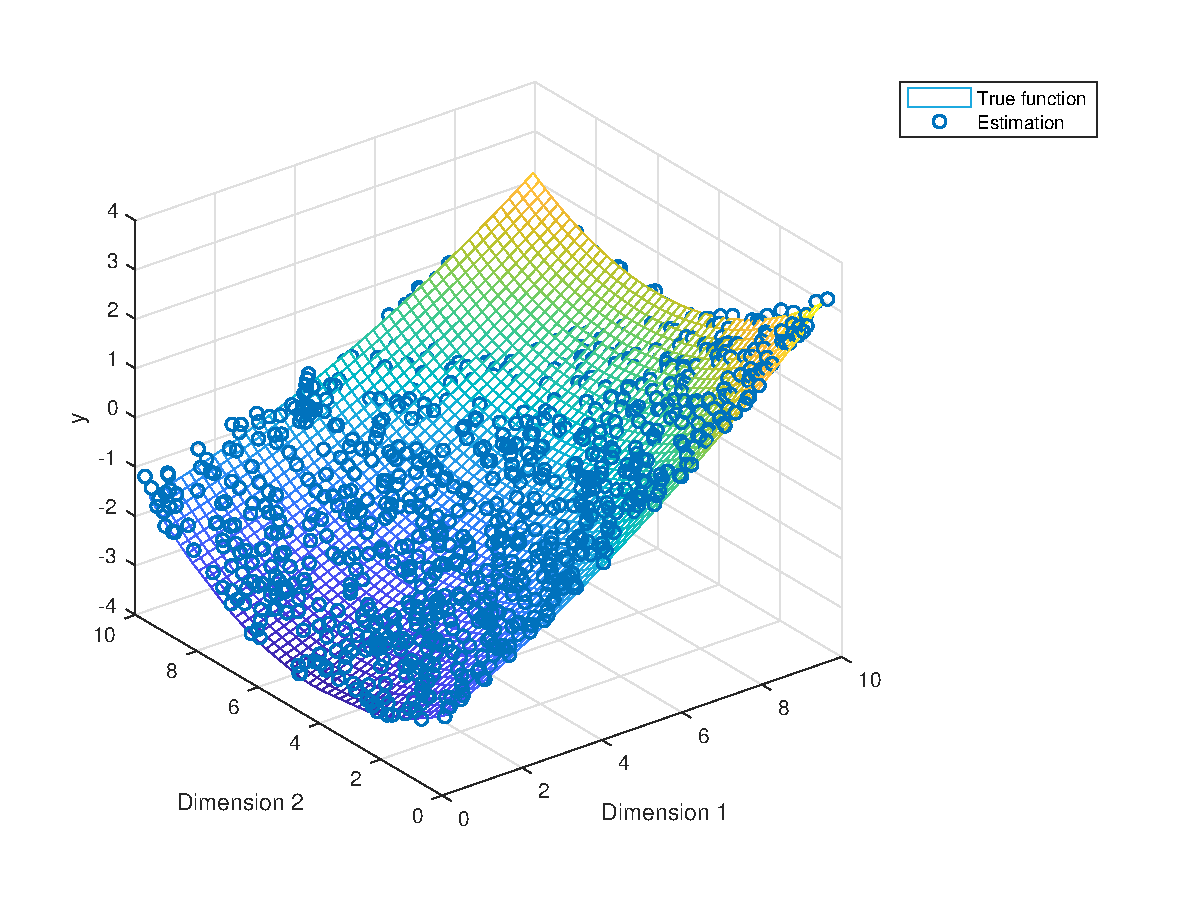
\includegraphics[scale=0.4]{project41c1}
	\caption{twoDimData1}
	\label{fig:twoDimData1-LR}
\end{subfigure}
\begin{subfigure}{.49\textwidth}
	\centering
	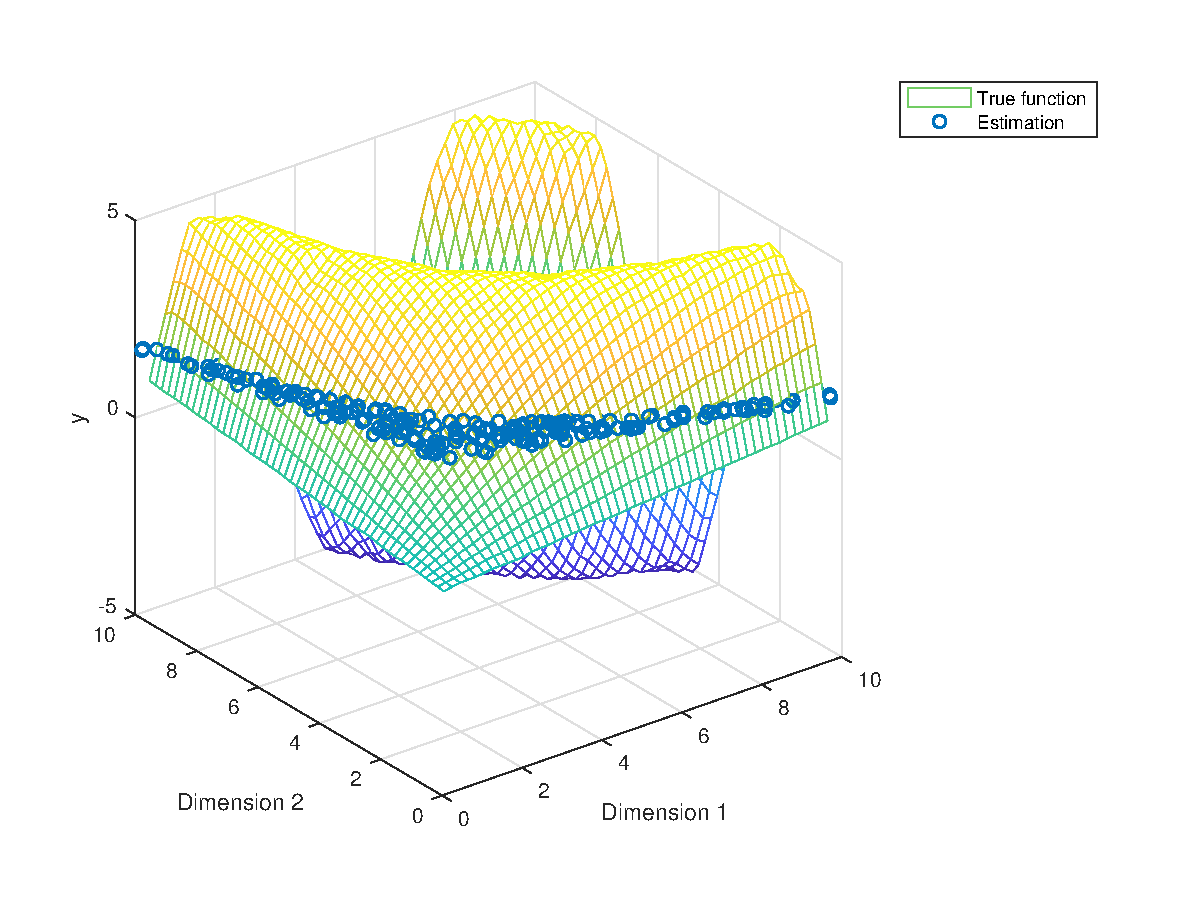
\includegraphics[scale=0.4]{project41c2}
	\caption{twoDimData2}
	\label{fig:twodimData2-LR}
\end{subfigure}
\caption{Linear regression on two data sets.}
\label{fig:twoDimData-LR}
\end{figure}


\subsubsection{Polynomial models}
In Figure \ref{fig:proj1-4_1d-degree} the mean square error for varying degrees of polynomials is presented. Best regression results are obtained using polynomials of degree 2 for twoDimData1 and polynomials of degree 4 for twoDimData2.

\begin{figure}[ht]
\centering
\begin{subfigure}{.49\textwidth}
	\centering
	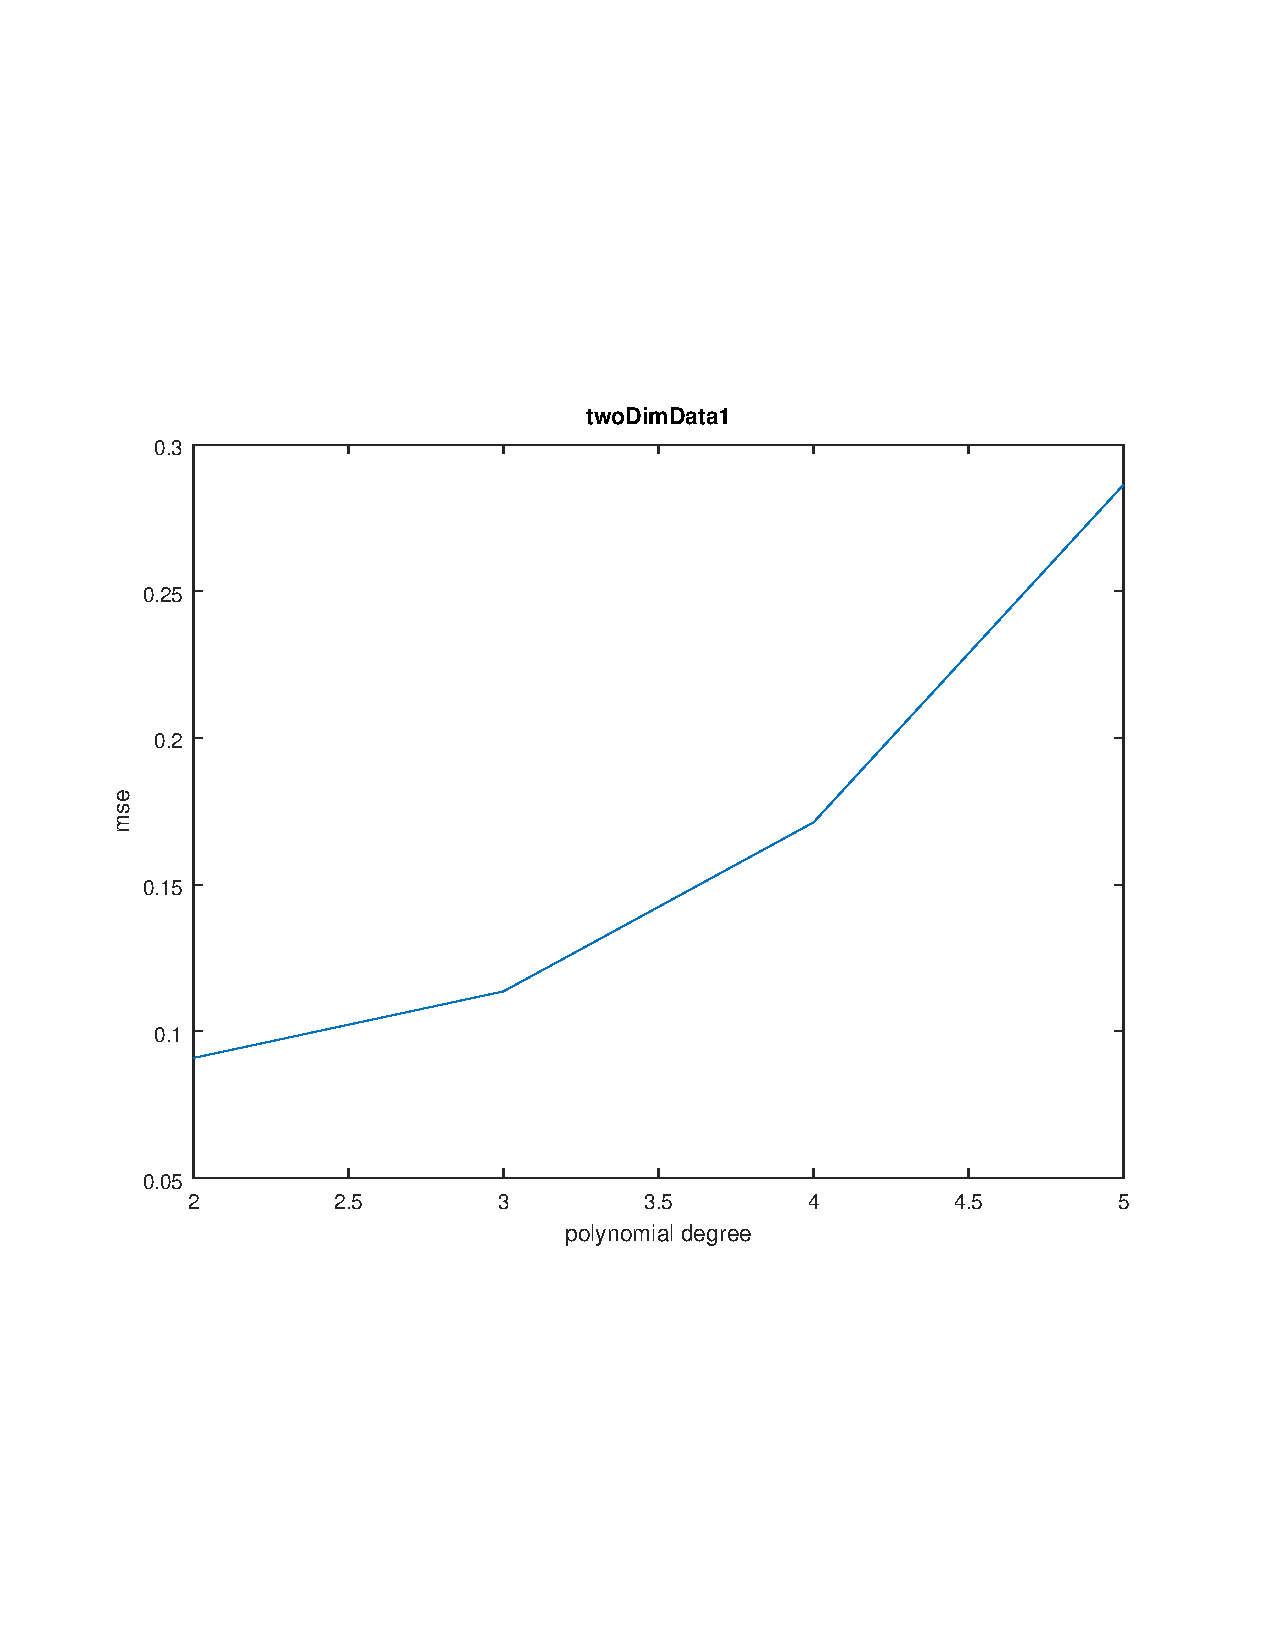
\includegraphics[trim= 10cm 5cm 10cm 5cm, scale=0.4]{proj1-4_1d-degree-data1}
	\caption{twoDimData1}
	\label{proj1-4_1d-degree-data1}
\end{subfigure}
\begin{subfigure}{.49\textwidth}
	\centering
	\includegraphics[trim= 10cm 5cm 10cm 5cm, scale=0.4]{proj1-4_1d-degree-data2}
	\caption{twoDimData2}
	\label{proj1-4_1d-degree-data2}
\end{subfigure}
\caption{Mean square error VS degree of polynomials in polynomial regression for two data sets.}
\label{fig:proj1-4_1d-degree}
\end{figure}

\ifx
\begin{table}[hb]
	\centering
	\caption{Mean square error}
	\label{tab:twodimData}
	\begin{tabular}{@{}ccccc@{}}
		\toprule
		Polynomial degree & 2   & 3   & 4   & 5   \\ \midrule
		twoDimData1       & 0.1 & 0.2 & 0.3 & 0.4 \\
		twoDimData2       & 8.5 & 5.0 & 4.2 & 2.9 \\ \bottomrule
	\end{tabular}
\end{table}
\fi

\subsubsection{KNN model}

\begin{figure}[ht]
\centering
\begin{subfigure}{.49\textwidth}
	\centering
	\includegraphics[trim= 10cm 5cm 10cm 5cm, scale=0.4]{proj1-4_1e-mse-data1}
	\caption{twoDimData1}
	\label{fig:proj1-4_1e-mse-data1}
\end{subfigure}
\begin{subfigure}{.49\textwidth}
	\centering
	\includegraphics[trim= 10cm 5cm 10cm 5cm, scale=0.4]{proj1-4_1e-mse-data2}
	\caption{twoDimData2}
	\label{fig:proj1-4_1e-mse-data2}
\end{subfigure}
\caption{Mean square error VS number of neighbors for a KNN regressor for two different data sets.}
\label{fig:proj1-4_1e-mse}
\end{figure}
\textbf{twoDimData1}: Given 100 generated data, the KNN model gives the best estimation result when choosing the number of neighbors around $K=10$ (see Figure \ref{fig:proj1-4_1e-mse-data1}), and the polynomial model outperforms the KNN. Increasing the number of data will not change the comparison result. However, when the data size is very small, e.g., 10, both the polynomial model and the KNN cannot provide a good estimation. In this case, which model is better depends on the stochastically generated data.

\textbf{twoDimData2}: Given 100 generated data, the KNN model gives the best estimation result when choosing the number of neighbors around $K=3$ (see Figure \ref{fig:proj1-4_1e-mse-data2}), and the KNN outperforms the polynomial model. Empirical results show that increasing or decreasing the number of data may influence the optimal number of neighbors but will not change the comparison result.

\subsection{Ten dimensional data} 

\subsubsection{Number of regressors}
Given a ten dimensional data, a linear regression model has 11 regressors, one for constant, and ten for linear terms. For a linear regression of polynomials up to degree 3 this is a bit more complicated. The formula ${r+n-1}\choose{r}$, which gives the number of combinations to choose $r$ items among $n$ items \textbf{with replacement} will be used to verify that the number of regressors is 286. There is 1 constant regressor, ${1+10-1}\choose{1}$ = 10 linear regressors, ${2+10-1}\choose{2}$ = 55 quadratic regressors, and ${3+10-1}\choose{3}$ = 220 qubic regressors, giving a total of 1+10+55+220=286. This match the number of regressors in our implemented code.

\subsubsection{Testing result of linear regression model}
A linear regression model outperforms a polynomial model with degree 3 without regularization. Adding regularization to the polynomial model can improve the estimation performance substantially, see Figure \ref{fig:proj1-4_2e-regul}.

 \begin{figure}[ht]
	\centering
	\includegraphics[trim= 10cm 5cm 10cm 5cm, scale=0.4]{proj1-4_2e-regul}
	\caption{Regularization on linear regression models of polynomials of degree 1 and 3 given in the legend.}
	\label{fig:proj1-4_2e-regul}
\end{figure}

\subsubsection{Testing result of KNN}

 \begin{figure}[ht]
	\centering
	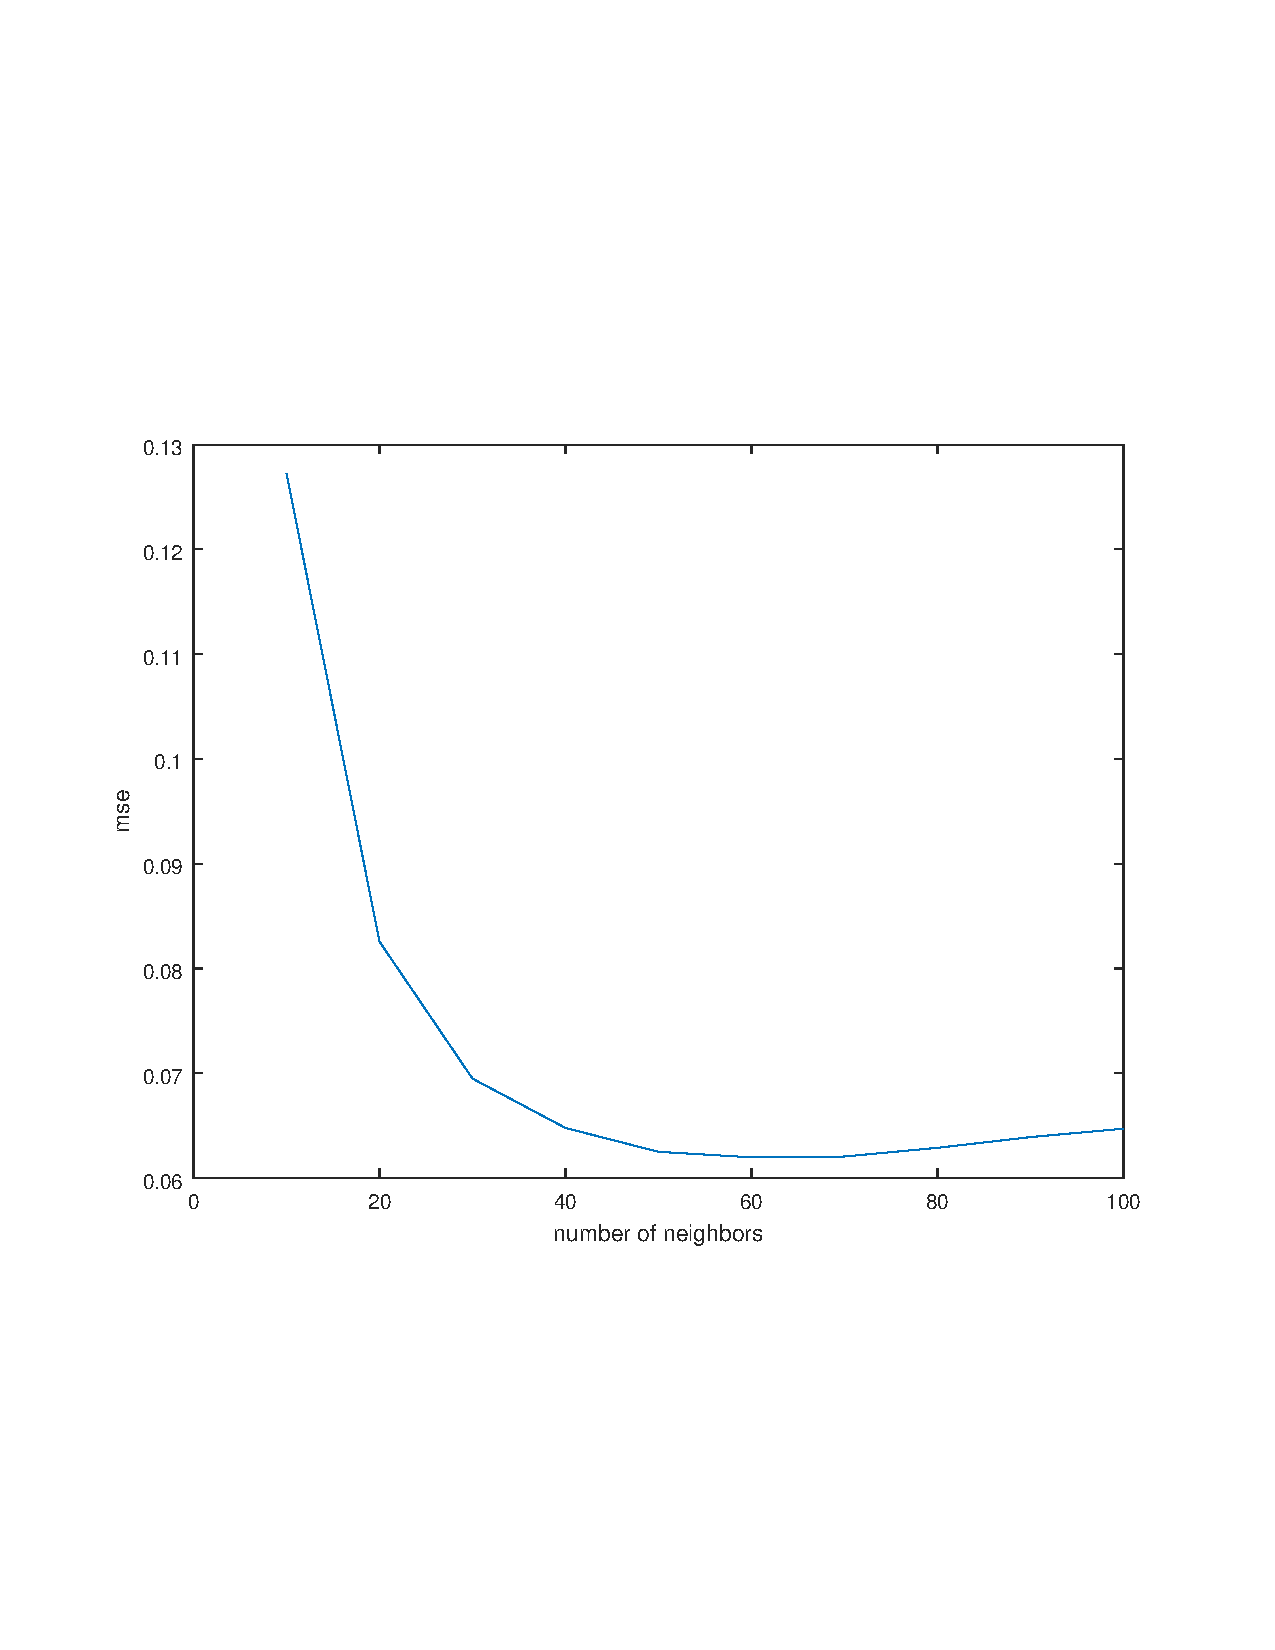
\includegraphics[trim= 10cm 5cm 10cm 5cm, scale=0.4]{proj1-4_2e-KNN}
	\caption{Number of neighbours for KNN regressor on 10 dimensional data.}
	\label{fig:proj1-4_2e-KNN}
\end{figure}

In Figure \ref{fig:proj1-4_2e-KNN} it can be seen that given 1000 data choosing the number of neighbors around $K=50$ gives the best result, and the linear regression with polynomial degree 3 and regularization parameter $\lambda=10$ outperforms the KNN. The best model however is the linear model using only polynomials to the degree 1 and regularization parameter 1. Increasing the data size will not change the comparison result. However, we found that, when the data size decreases to 500, KNN and linear regression start to have similar performance, and that, if we further decrease the data size, KNN will instead outperform linear regression.

\textbf{Analysis}:  As a general rule, linear regression will tend to outperform KNN when there is a small number of observations per predictor. This rule especially holds for high-dimensional data since the KNN suffers from the curse of dimensionality. However, our observation obeys this general rule. In the regression, we use all the possible regressors up to degree 3 to fit the model. However, it is more often the case that the response is only related to a subset of the regressors. In order to fit a single model involving regressors that are associated with the response, variable selection should have been done. Using redundant regressors will increase the chance to fit unexpected pattern in the data that are randomly generated by noise; thus estimation performance might be deteriorated. This explains our observation that the KNN outperforms the linear regression model without variable selection  even when the data size is small. 




\end{document}
